\section{Vector-Boson-Fusion process\footnote{A.~Denner, S.~Farrington,
  C.~Hackstein, C.~Oleari, D.~Rebuzzi (eds.); P.~Bolzoni, S.~Dittmaier, F.~Maltoni,
  S.-O.~Moch, A.~M\"uck, S. Palmer and M.~Zaro.} }

\providecommand{\lsim}
{\;\raisebox{-.3em}{$\stackrel{\displaystyle <}{\sim}$}\;}
\providecommand{\gsim}
{\;\raisebox{-.3em}{$\stackrel{\displaystyle >}{\sim}$}\;}

\subsection{Higgs-boson production in vector-boson fusion}
\label{sec:intro}
The production of a Standard Model Higgs boson in association with two hard
jets in the forward and backward regions of the detector, frequently quoted
as the ``vector-boson fusion''~(VBF) channel, is a cornerstone in
the Higgs-boson search both in the ATLAS~\cite{Asai:2004ws} and
CMS~\cite{Abdullin:2005yn} experiments at the LHC.  Higgs-boson production in
the VBF channel plays also an important role in the determination of
Higgs-boson couplings at the LHC (see e.g.,\ \Bref{Duhrssen:2004cv}). Bounds on
non-standard couplings between Higgs and electroweak~(EW) gauge bosons can be
imposed from precision studies in this channel~\cite{Hankele:2006ma}.
In addition this channel contributes in a significant way to the inclusive Higgs 
production over the full Higgs-mass range.

The production of a Higgs boson~+~2~jets receives two contributions at hadron
colliders. The first type, where the Higgs boson couples to a weak boson that
links two quark lines, is dominated by $t$- and $u$-channel-like diagrams and
represents the genuine VBF channel.  The hard jet pairs have a strong
tendency to be forward--backward directed in contrast to other jet-production
mechanisms, offering a good background suppression (transverse-momentum and
rapidity cuts on jets, jet rapidity gap, central-jet veto, etc.). 

If one is interested in the measurement of the Higgs-boson couplings in VBF,
especially for the measurement of the $\PH\PW\PW$ and $\PH\PZ\PZ$ couplings, 
cuts should
be applied in order to suppress events from Higgs~+~2~jet production via
gluon fusion, which become a background to the signal VBF production.  In the
gluon-fusion channel, the Higgs boson is radiated off a heavy-quark loop that
couples to any parton of the incoming hadrons via
gluons~\cite{DelDuca:2001fn,Campbell:2006xx}. Although the final states are
similar, the kinematic distributions of jets are very different.  Applying
appropriate event selection criteria, called VBF cuts (see
e.g.,\ \Brefs{Barger:1994zq, Rainwater:1997dg, Rainwater:1998kj,
  Rainwater:1999sd, DelDuca:2006hk}), it is possible to sufficiently suppress
the gluon-fusion Higgs-boson production mechanism with respect to the VBF
one.  According to a recent estimate~\cite{Nikitenko:2007it}, gluon fusion
contributes about $4{-}5\%$ to the Higgs~+~2~jet events for a Higgs-boson
mass of $120$\UGeV, after applying VBF cuts.
A next-to-leading order~(NLO)
analysis of the gluon-fusion contribution~\cite{Campbell:2006xx} shows that its residual
scale dependence is still of the order of $35\%$.

%Higgs-boson production in the VBF channel is a pure EW process in leading
%order~(LO) involving only quark and antiquark parton distributions.  The
%topologies of the LO Feynman diagrams contribution to various partonic
%processes are shown in~\Figure~\ref{fig:VBFLOtops}. 
Electroweak Higgs-boson production at leading order~(LO) involve only quark
and antiquark initial states, $\Pq \Pq\to \Pq \Pq\PH$.  The topologies of the
LO Feynman diagrams contributing to various partonic processes are shown
in~\Figure~\ref{fig:VBFLOtops}.  As $s$-channel diagrams and interferences
tend to be suppressed when imposing VBF cuts, the cross section can be
approximated by the contribution of squared $t$- and $u$-channel diagrams only
without their interference.  The
corresponding QCD corrections reduce to vertex corrections to the
weak-boson--quark coupling.  Explicit NLO QCD calculations in this
approximation~\cite{Spira:1997dg,Han:1992hr,Figy:2003nv,Figy:2004pt,Berger:2004pca}
confirm the expectation that these QCD corrections are small, because they
are shifted to the parton distribution functions (PDFs) via QCD factorization
to a large extent. The resulting QCD corrections are of the order of
$5{-}10\%$ and reduce the remaining factorization and renormalization scale
dependence of the NLO cross section to a few percent.
%For the NLO QCD
%predictions from {\tt HAWK}~\cite{Ciccolini:2007jr,Ciccolini:2007ec,HAWK},
%{\tt VBFNLO}~\cite{Figy:2003nv,Arnold:2008rz} and VV2H~\cite{VV2H}, which
%calculates only total cross sections without cuts, a tuned comparison has
%been performed in~\cite{HiggsLH:2008uu} neglecting $s$-channel diagrams and
%interferences. The results of all three codes were found to agree within the
%statistical errors at the level of 0.1 per cent.
For the NLO QCD predictions from {\sc
  HAWK}~\cite{Ciccolini:2007jr,Ciccolini:2007ec,HAWK}, {\sc
  VBFNLO}~\cite{Figy:2003nv,Arnold:2008rz}, and {\sc VV2H}~\cite{VV2H} (this last
program calculates only total cross sections without cuts), a tuned
comparison has been performed in \Bref{HiggsLH:2008uu}, neglecting $s$-channel
diagrams and interferences. Recently, {\sc VBF@NNLO}~\cite{Bolzoni:2010xr}
was also run in the same setup.  The results of all four codes were found to
agree within the statistical errors at the level of $0.1\%$.


\newcommand\scalefac{0.9}
\newlength{\largfig}
\largfig=\scalefac pt

\begin{figure}
  \begin{center}
    {\unitlength \largfig 
      \begin{picture}(125,130)(0,0)
        \SetScale{\scalefac}
        \Line( 15,95)( 65,90)
        \Line( 15, 5)( 65,10)
        \Line(115, 5)( 65,10)
        \Line(115,95)( 65,90)
        \Photon( 65,10)( 65,90){3}{7}
        \DashLine(115,50)( 65,50){6}
        \Vertex(65,90){2}
        \Vertex(65,10){2}
        \Vertex(65,50){2}
        \put(  0,90){$\Pq$}
        \put(  0,0){$\Pq$}
        \put(123,90){{$\Pq$}}
        \put(123,0){{$\Pq$}}
        \put(123,45){{$\PH$}}
        \put( 75,65){{$V$}}
        \put( 75,20){{$V$}}
        \SetScale{1}
      \end{picture}
    }%
    \hspace*{2em}%
            {\unitlength  \largfig 
              \begin{picture}(125,100)(0,0)
                \SetScale{\scalefac}
                \Line( 15,95)( 65,10)
                \Line( 15, 5)( 65,90)
                \Line(115, 5)( 65,10)
                \Line(115,95)( 65,90)
                \Photon( 65,10)( 65,90){3}{7}
                \DashLine(115,50)( 65,50){6}
                \Vertex(65,90){2}
                \Vertex(65,10){2}
                \Vertex(65,50){2}
                \put(  0,90){$\Pq$}
                \put(  0,0){$\Pq$}
                \put(123,90){{$\Pq$}}
                \put(123,0){{$\Pq$}}
                \put(123,45){{$\PH$}}
                \put( 75,65){{$V$}}
                \put( 75,20){{$V$}}
                \SetScale{1}
              \end{picture}
            }%
            \hspace*{2em}%
                    {\unitlength  \largfig  
                      \begin{picture}(145,100)(0,0)
                        \SetScale{\scalefac}
                        \Line( 15,95)( 35,50)
                        \Line( 15, 5)( 35,50)
                        \Line(135,95)(115,50)
                        \Line(135, 5)(115,50)
                        \Photon( 35,50)(115,50){3}{7}
                        \DashLine(75,50)(95,95){6}
                        \Vertex( 35,50){2}
                        \Vertex(115,50){2}
                        \Vertex( 75,50){2}
                        \put(  0,90){$\Pq$}
                        \put(  0,0){$\Pq$}
                        \put(143,90){{$\Pq$}}
                        \put(143,0){{$\Pq$}}
                        \put(103,90){{$\PH$}}
                        \put( 45,30){{$V$}}
                        \put( 85,30){{$V$}}
                        \SetScale{1}
                      \end{picture}
                    }                      
  \end{center}
  \caption{Topologies of $t$-, $u$-, and $s$-channel contributions
for electroweak Higgs-boson production, $\Pq
    \Pq\to \Pq \Pq\PH$ at LO, where $\Pq$ denotes any quark or antiquark and
    $V$ stands for \PW and \PZ~boson.}
  \label{fig:VBFLOtops}
\end{figure}

In \Brefs{Ciccolini:2007jr,Ciccolini:2007ec} the full NLO EW +
QCD corrections have been computed with {\sc HAWK}, including the complete set of
$t$-, $u$-, and $s$-channel Feynman diagrams and taking into account
real corrections induced by photons in the initial state and QED
corrections implicitly contained in the DGLAP evolution of PDFs.  The
size of the electroweak corrections sensitively depends on the chosen
renormalization scheme to define the weak couplings, most notably on
the chosen value for the electromagnetic coupling $\alpha$. The
preferred choice, which should be most robust with respect to
higher-order corrections, is the so-called $\GF$ scheme, where
$\alpha$ is derived from Fermi's constant $\GF$.  The impact of EW and
QCD corrections in the favoured Higgs-mass range between $100$ and
$200$\UGeV{} are of order $5\%$ and negative, and thus as important as
the QCD corrections.  Photon-induced processes lead to corrections at
the percent level.

Approximate next-to-next-to-leading order~(NNLO) QCD corrections to the total
inclusive cross section for VBF have been presented in \Bref{Bolzoni:2010xr}.
The theoretical predictions are obtained using the structure-function
approach~\cite{Han:1992hr}. Upon including the NNLO corrections in QCD for
the VBF production mechanism via the structure-function approach the
theoretical uncertainty for this channel, i.e. the scale dependence, reduces from the $5{-}10\%$ of the
NLO QCD and electroweak combined
computations~\cite{Han:1992hr,Ciccolini:2007ec} down to $1{-}2\%$. The
uncertainties due to parton distributions are estimated to be at the same
level.




\subsection{Higher-order calculations}
\label{sec:NLO_calculations}
In order to study the NLO corrections to Higgs-boson production in VBF, we
have used two existing partonic Monte Carlo programs: {\sc HAWK} and {\sc
  VBFNLO}, which we now present. Furthermore we also give results of the
NNLO QCD calculation based on {\sc VBF@NNLO} and combine them with the
electroweak corrections obtained from {\sc HAWK}.

\subsubsection{HAWK -- NLO QCD and EW corrections}
\label{sec:HAWK}
{\sc HAWK}~\cite{Ciccolini:2007jr,Ciccolini:2007ec,HAWK} is a Monte Carlo
event generator for $\Pp\Pp\to\PH + 2\,\mathrm{jets}$.  It includes the
complete NLO QCD and electroweak corrections and all weak-boson fusion and
quark--antiquark annihilation diagrams, i.e.~$t$-channel and $u$-channel
diagrams with VBF-like vector-boson exchange and $s$-channel Higgs-strahlung
diagrams with hadronic weak-boson decay.  Also, all interferences at LO and
NLO are included. If it is supported by the PDF set, contributions from
incoming photons, which are at the level of $1{-}2\%$, can be taken into
account.  Leading heavy-Higgs-boson effects at two-loop order proportional to
$\GF^2 \MH^4$ are included according to
\Brefs{Ghinculov:1995bz,Frink:1996sv}. While these contributions are
negligible for small Higgs-boson masses, they become important for
Higgs-boson masses above $400$\UGeV.  For $\MH=700$\UGeV{} they yield
$+4\%$, i.e.~about half of the total EW corrections. This signals a breakdown
of the perturbative expansion, and these contributions can be viewed as an
estimate of the theoretical uncertainty.  Contributions of $\PQb$-quark PDFs
and final-state $\PQb$ quarks can be taken into account at LO. While the
effect of only initial $\PQb$ quarks is negligible, final-state $\PQb$ quarks can increase the cross section by up to $4\%$.
While $s$-channel diagrams can contribute up to $25\%$ for small
Higgs-boson masses in the total cross section without cuts, their contribution is below
 $1\%$ once VBF cuts are applied. Since the $s$-channel diagrams are
actually a contribution to $\PW\PH$ and $\PZ\PH$ production, they
are switched off in the following.

The code is interfaced to LHAPDF and allows to evaluate
the PDF uncertainties in a single run.  The calculation can be performed for an
on-shell Higgs boson or for an off-shell Higgs boson decaying into a pair of
gauge singlets, thus mimicking an off-shell Higgs boson. While the effects of
the off-shellness are negligible for small Higgs-boson masses, they should be
taken into account for $\MH \gsim 400$\UGeV. As a flexible partonic Monte
Carlo generator, {\sc HAWK} allows to apply phase-space cuts on the jets and
the Higgs-boson decay products and to switch off certain contributions.


\subsubsection{VBFNLO -- NLO QCD and EW corrections}
\label{sec:VBFNLO}
{\sc VBFNLO}~\cite{webVBFNLO} is a fully flexible partonic Monte Carlo
program for VBF, double and triple vector-boson production processes at NLO
QCD accuracy.  Arbitrary cuts can be specified as well as various scale
choices: in fact, {\sc VBFNLO} can use fixed or dynamical renormalization and
factorization scales. Any currently available parton distribution function
set can be used through the LHAPDF library.  For processes implemented at
leading order, the program is capable of generating event files in the Les
Houches Accord (LHA) format~\cite{Alwall:2006yp}.

Since, in the phase-space regions which are accessible at hadron colliders,
VBF reactions are dominated by $t$-channel electroweak gauge-boson exchange,
in {\sc VBFNLO}, $s$-channel exchange contributions and
kinematically-suppressed fermion-interference
contributions~\cite{Andersen:2007mp,Bredenstein:2008tm} are disregarded. 
While the interference
effects are always well below $1\%$, they are entirely negligible once VBF
cuts are applied. Here, even the $s$-channel contributions which, with
excellent accuracy, can be regarded as a separate "Higgs-strahlung" process, drop below 1\%.
The subsequent decay of the Higgs boson is simulated in the narrow-width
approximation.  For the $\PH\to \PW^+\PW^- $ and the $\PH\to \PZ\PZ$ modes,
full off-shell effects and spin correlations of the decay leptons are
included.  Details of the calculation can be found in
\Bref{Figy:2003nv}.  Very recently, the EW corrections to VBF
Higgs-boson production have been added to the code~\cite{Figy:2010ct}.

%For completeness, we point out here that study of the $s$-channel
%contribution is better addressed in the $VH$ session, when considering the
%hadronic decay of the vector boson $V$.

\subsubsection{VBF@NNLO -- NNLO QCD corrections}
\label{sec:VBF-NNLO}

%========================================================================
% original version of Moch/Maltoni

%The structure function approach~\cite{Han:1992hr} consists basically in
%viewing the VBF process as a double deep-inelastic scattering (DIS) attached
%to the colorless pure electroweak vector boson fusion into a Higgs boson. A
%qualitative illustration of the structure function approach is given in
%fig.~\ref{fig:strucfuncapp}.  According to this approach one can include NLO
%QCD corrections to the VBF process employing the standard DIS structure
%functions $F_i(x,Q^2);\,i=1,2,3$ at NLO~\cite{Bardeen:1978yd}.  Similarly at
%the NNLO level one has to employ the corresponding structure
%functions~\cite{Kazakov:1990fu,Zijlstra:1992kj,Zijlstra:1992qd,Moch:1999eb}.
%
%\begin{figure}[htb]
%\vspace{5pt}
%\centering
%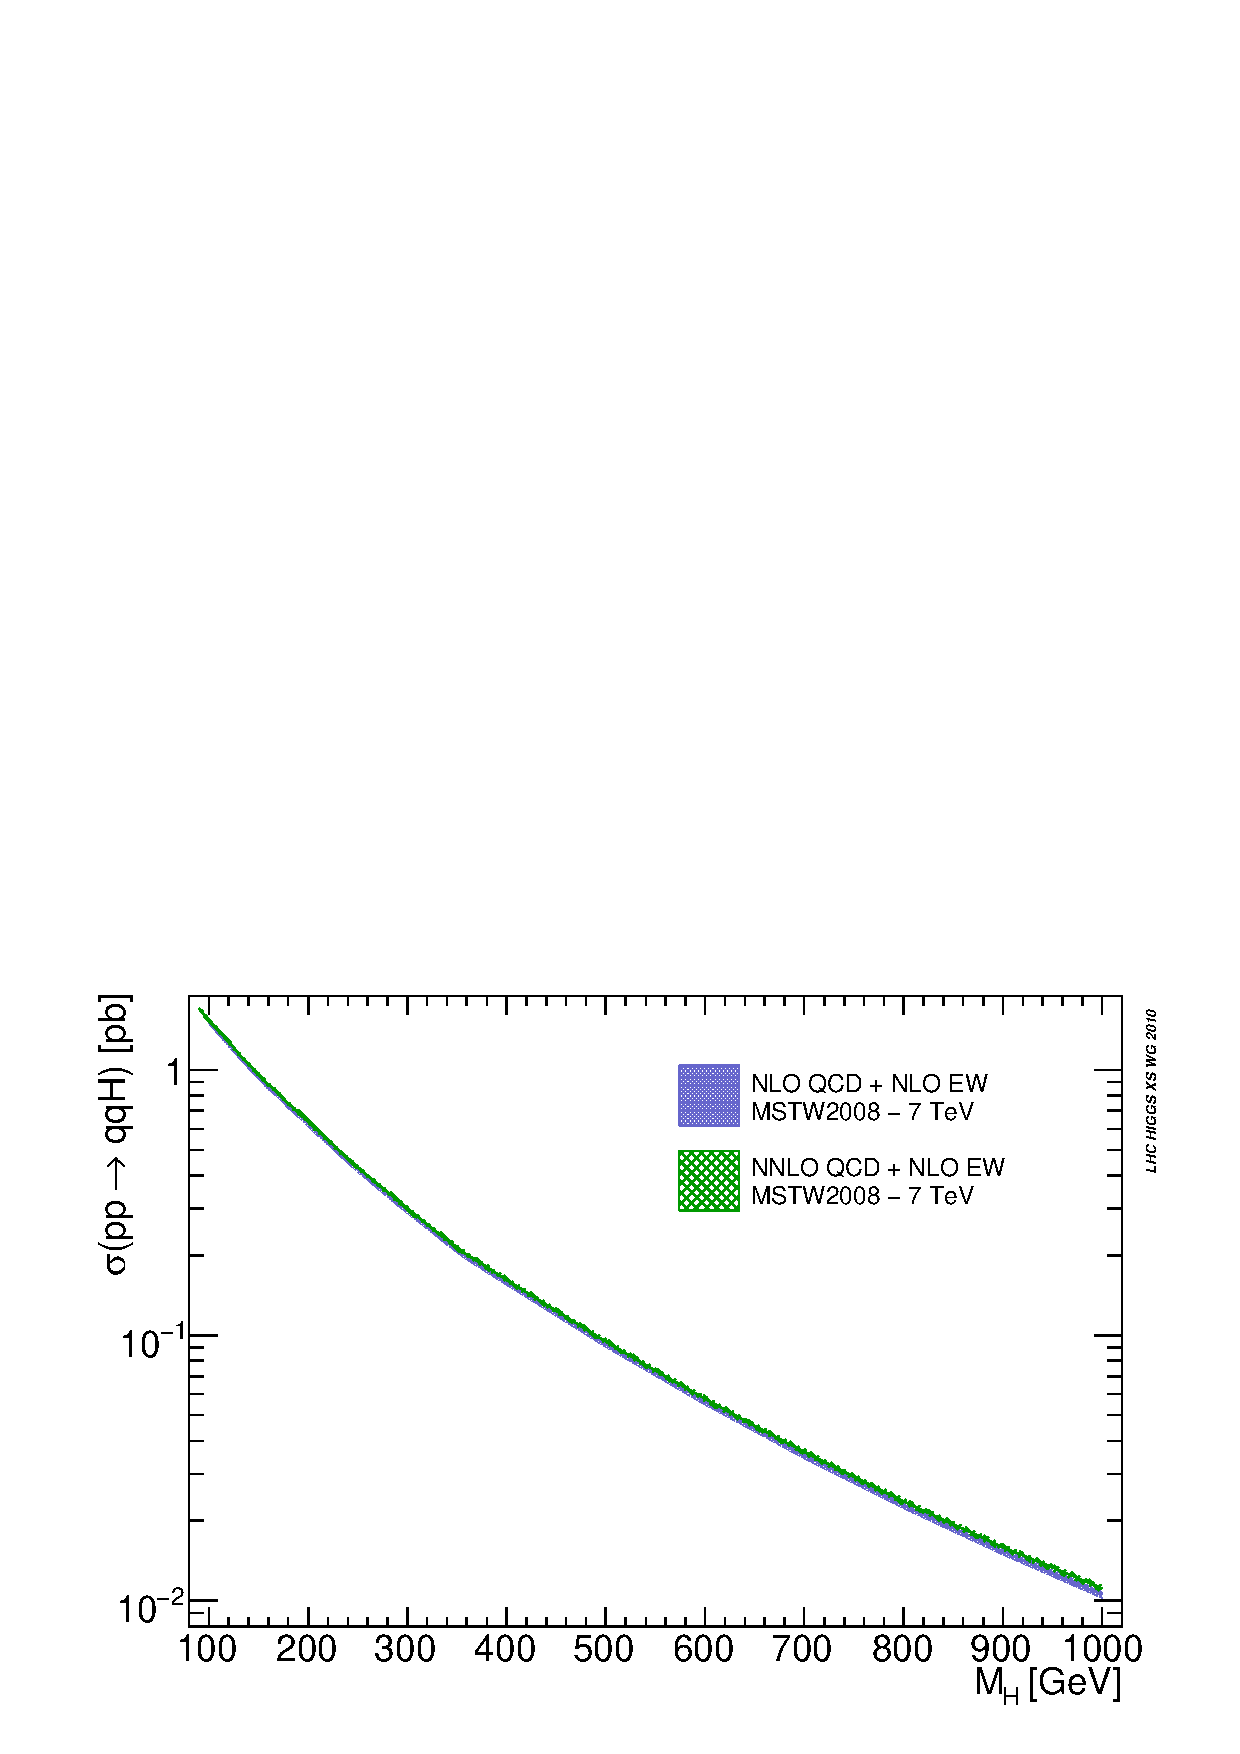
\includegraphics[width=.5\linewidth]{YRHXS_VBF/YRHXS_VBF_fig1}
%%\vspace*{-15pt}
%\caption{Schematic view of the structure function approach.}
%\label{fig:strucfuncapp}
%\end{figure}
%
%The structure function approach represents a very accurate approximation
%because it is based on the absence or smallness of the QCD interference
%contributions between the two inclusive final states $X_1$ and $X_2$. We now
%discuss the various contributions up to NNLO which in principle violate the
%structure function approach but which can nevertheless be safely neglected.
%
%At LO there is already a structure function violating contribution coming
%from the interferences between identical final state quarks
%(e.g.\ $uu\rightarrow Huu$) or between processes where either a $\PW$ or a $Z$
%can be exchanged (e.g.\ $ud\rightarrow Hud$). Simple kinematical arguments
%show that such contributions are very small and contribute to the total cross
%section well below the percent level~\cite{Dicus:1985zg}.  These
%contributions can be easily computed and have been included in our results
%anyway.
%
%At the NLO level possible contributions violating the structure function
%approach arise when a gluon in the $t$-channel is exchanged between the
%initial quarks of the two incident protons.  However the interference of such
%one-loop contributions with the LO diagram have a vanishing color
%factor. This means that apart from the interference effects discussed at LO
%the structure function approach represents an exact approach to the
%computation.
%
%\begin{figure}[htb]
%\centering
%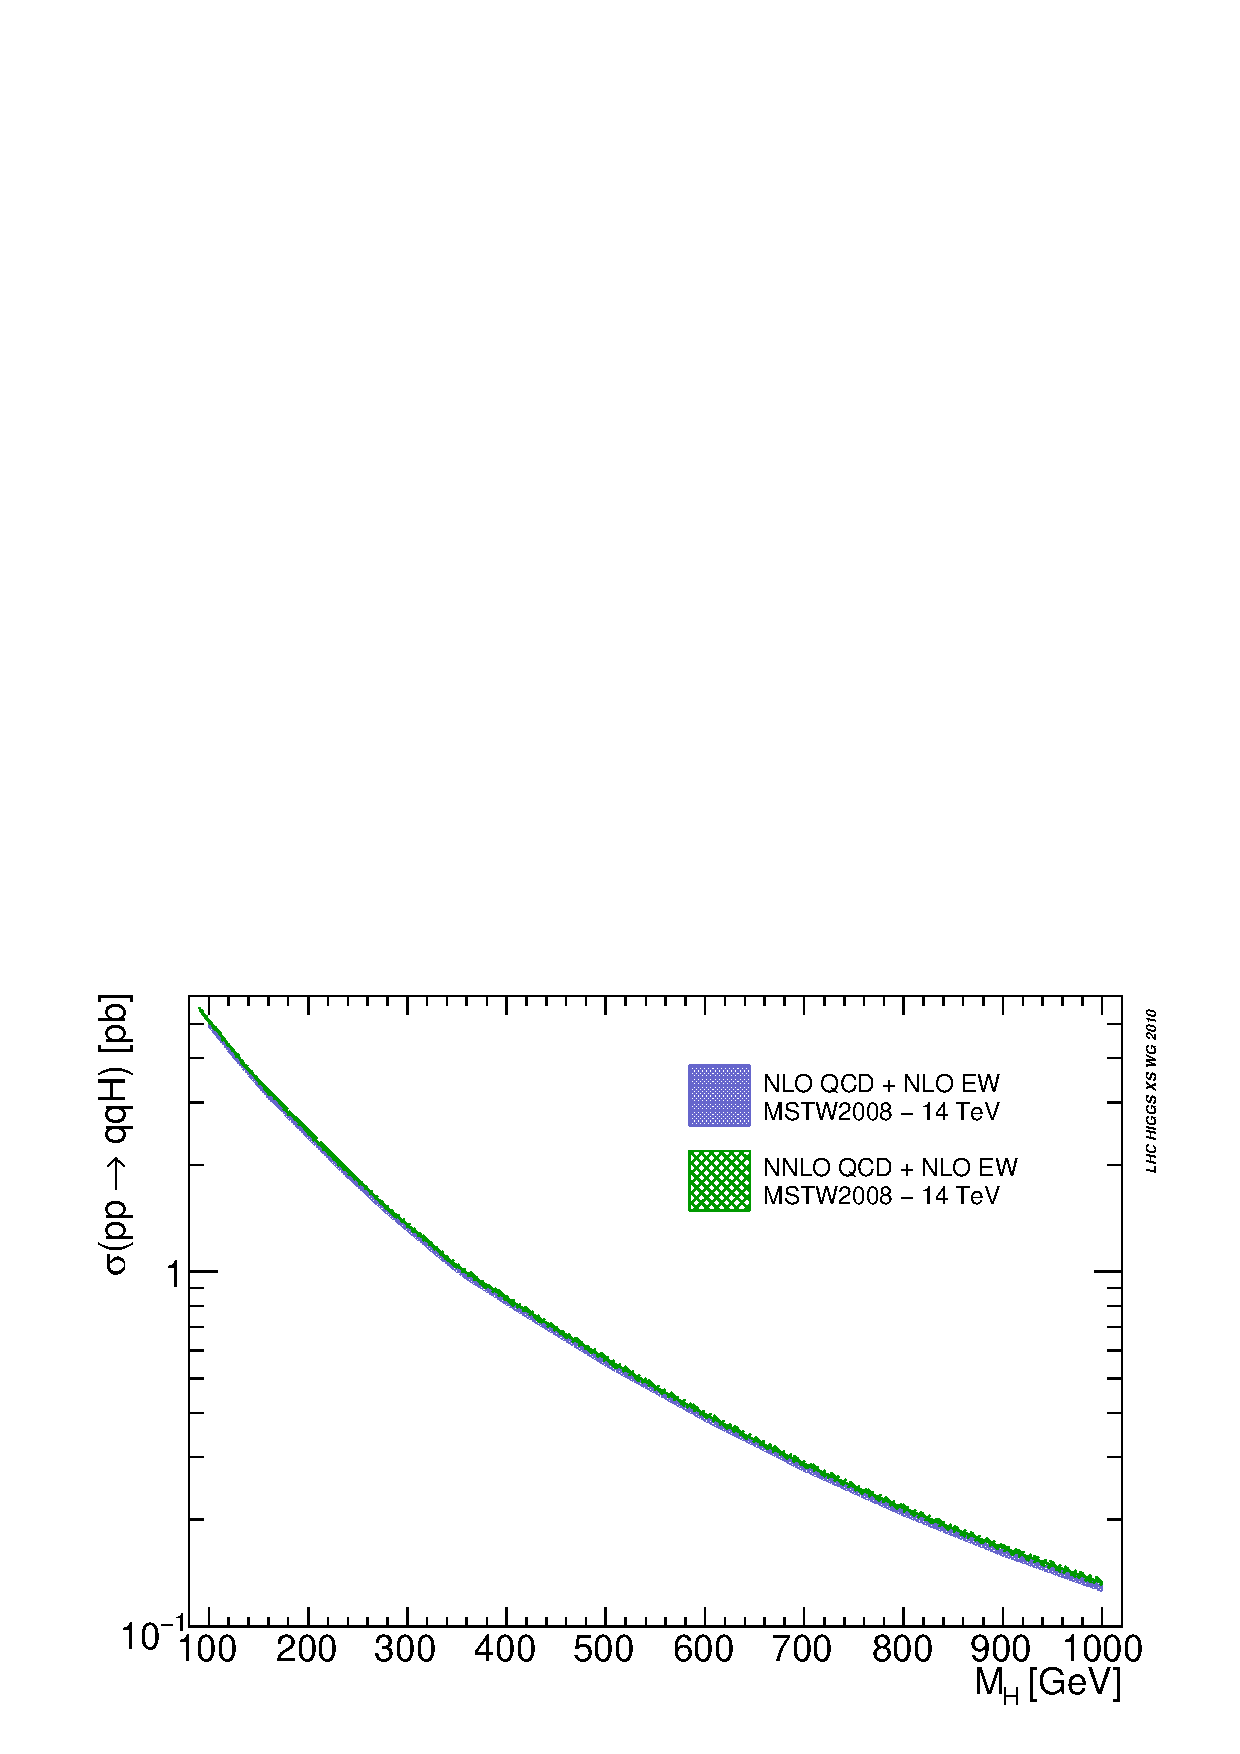
\includegraphics[width=.5\linewidth]{YRHXS_VBF/YRHXS_VBF_fig2}
%%\vspace*{-15pt}
%\caption{Examples of neglected Feynman diagrams at NNLO.}
%\label{fig:neglect}
%\end{figure}
%
%At NNLO the structure function approach is not exact but it can be still
%considered a very good approximation.  The types of diagrams that violate the
%structure function approach are shown in fig.~\ref{fig:neglect}. The first
%type represents a double gluon-exchange in the $t$-channel (note that one or
%both of the two emissions could also be real); the second type is a
%representative of the so-called single quark line (SQL) diagrams contributing
%at NNLO; the last two are heavy quarks (top and bottom) loop diagrams. The
%first type of contributions represents a gauge invariant, infrared and
%ultraviolet finite class of diagrams. Another characteristic of this class of
%diagrams is its color suppression by a factor of $1/N_c^2$ with respect to
%the contributions included by the structure function approach. Furthermore
%this type of contributions are also strongly kinematically
%suppressed~\cite{vanNeerven:1984ak,Blumlein:1992eh,Figy:2007kv}.  This is
%mainly due to the behavior of the gluon propagator in the $t$-channel and/or
%to the small overlapping of the phase space of real emissions from the upper
%quark line and real emissions from the lower one.  The neglected SQL type
%contributions in fig.~\ref{fig:neglect} do not represent a class of infrared
%safe diagrams. However as shown in~\cite{Harlander:2008xn} their impact is
%small enough not to produce a significant deterioration of the VBF signal.
%A first rough estimation for the triangle (evaluated in the limit of infinite
%top mass) and for the box contributions in fig.~\ref{fig:neglect} showed that
%their contribution is small and can be safely neglected.
%
%The LO, NLO and NNLO results in QCD are shown as a function of the Higgs
%boson mass.  The theoretical uncertainty of the predictions have been
%obtained by varying the factorization and the renormalization scales in the
%range $\mu_{\rm{R(F)}}\in [Q/4,4Q]$ where $Q$ is the virtuality of the vector
%bosons which ``fuse'' into the Higgs.  Clearly other scale choices are
%possible (e.g. $\mu_{\rm{R(F)}}\in [\MH/4,4\MH]$ with the Higgs mass $\MH$ or
%$\mu_{\rm{R(F)}}\in [\MW/4,4\MW]$ with the $\PW$-boson mass $\MW$) but the
%recommend one, i.e.~$\mu_{\rm{R(F)}}\in [Q/4,4Q]$, turned out to be the more
%natural choice because it exhibits a better convergence of the perturbative
%expansion.  This also shows that at NNLO in QCD the theoretical uncertainty
%is reduced to be less than the $2\%$ reaching the same level of ambiguity at
%which the Higgs production signal via VBF can be defined phenomenologically.
%
%We also consider the uncertainties coming from the parton distributions.  To
%achieve this we have employed the MSTW $68\%$ confidence level PDF
%sets~\cite{Martin:2009iq} and compared with other NNLO PDF sets,
%i.e.\ ABKM~\cite{Alekhin:2009ni} and JR09VF~\cite{JimenezDelgado:2009tv}. The
%results show that an almost constant $2\%$ PDF uncertainty can be associated
%to the cross section for the LHC.
%
%All numbers presented here can also be obtained via the web interface where
%the code for the NNLO VBF total cross section can be used
%online~\cite{WebInterface:2010}. 
%===========================================================================
{\sc VBF@NNLO}~\cite{Bolzoni:2010xr} computes VBF Higgs cross sections 
at LO, NLO, and NNLO in QCD via the structure-function approach.  This
approach~\cite{Han:1992hr} consists basically in viewing the VBF process as a
double deep-inelastic scattering (DIS) attached to the colourless pure
electroweak vector-boson fusion into a Higgs boson.  According to this
approach one can include NLO QCD corrections to the VBF process employing the
standard DIS structure functions $F_i(x,Q^2);\,i=1,2,3$ at
NLO~\cite{Bardeen:1978yd} or similarly the corresponding structure
functions~\cite{Kazakov:1990fu,Zijlstra:1992kj,Zijlstra:1992qd,Moch:1999eb}.

The structure-function approach does not include all types of contributions.
At LO a structure-function-violating contribution comes from the
interferences between identical final-state quarks (e.g.,\
$\PQu\PQu\rightarrow \PH\PQu\PQu$) or between processes where either a $\PW$
or a $\PZ$ can be exchanged (e.g.,\ $\PQu\PQd\rightarrow \PH\PQu\PQd$).  These
LI contributions have been included in the NNLO results. Apart from such
contributions, the structure-function approach represents an exact approach
also at NLO.  At NNLO, however, several types of diagrams violate it.  Some
are colour suppressed and kinematically
suppressed~\cite{vanNeerven:1984ak,Blumlein:1992eh,Figy:2007kv}, others have
been shown in \Bref{Harlander:2008xn} to be small enough not to produce
a significant deterioration of the VBF signal.  A first rough estimation for
a third set showed that their contribution is small and can be safely
neglected.  At NNLO in QCD, the theoretical uncertainty is reduced to be less
than $2\%$.


\subsection{Results}
In the following, we present VBF results for LHC at $7\UTeV$ and $14\UTeV$
calculated at NLO, from {\sc HAWK} and {\sc VBFNLO}~\cite{webVBFNLO}, and at
NNLO, from {\sc VBF@NNLO}~\cite{WebInterface:2010}.

All results have been computed using the values of the electroweak parameters
given in~\refA{sminput}. The renormalization and factorization scales have
been fixed to $\MW$, and both the scales varied in the range
$\MW/2<\mu<2\MW$. The Higgs boson has been treated as stable on on-shell, and
the contributions from $s$-channel diagrams have been neglected.

\begin{figure}
  \includegraphics[width=0.5\textwidth]{YRHXS_VBF/YRHXS_VBF_fig1.eps}
  \includegraphics[width=0.5\textwidth]{YRHXS_VBF/YRHXS_VBF_fig2.eps}
  \caption{VBF cross sections at the LHC at $7\UTeV$~(left) and $14\UTeV$ (right)
    estimated with MSTW2008 PDF set.  NLO QCD results and NNLO QCD
results are shown both with the
    EW corrections. The bands represent the
    PDF + $\alphas$ 68\% CL uncertainty.}
  \label{fig:totXsecMSTW2008}
\end{figure}

\begin{figure}
  \includegraphics[width=0.5\textwidth]{YRHXS_VBF/YRHXS_VBF_fig3.eps}
  \includegraphics[width=0.5\textwidth]{YRHXS_VBF/YRHXS_VBF_fig4.eps}
  \caption{NLO VBF cross sections at the LHC at $7\UTeV$~(left) and
    $14\UTeV$ (right). Results with and without the EW corrections
    are plotted. The bands represent the PDF + $\alphas$ 68\% CL uncertainty coming from
	 the {\em envelope} of three PDF sets (see text for details).}
  \label{fig:totXsecEnvelope}
\end{figure}

%\Figure~\ref{fig:totXsecMSTW2008} and \Figure~\ref{fig:totXsecEnvelope}
%summarize the VBF results at the LHC at $7$ and $14\UTeV$.  In
%\Figure~\ref{fig:totXsecMSTW2008}, the cross section results at NLO QCD, NNLO
%QCD, NLO QCD with EW corrections, and NNLO QCD with EW corrections are shown
%as a function of the Higgs-boson mass.  
Figures~\ref{fig:totXsecMSTW2008} and \ref{fig:totXsecEnvelope}
summarize the VBF results at the LHC at $7\UTeV$ and $14\UTeV$.  In
\Figure~\ref{fig:totXsecMSTW2008}, the cross section results at NLO
QCD and NNLO QCD both with EW corrections are shown
as a function of the Higgs-boson mass.
Calculations are performed with the
MSTW2008 68\% CL PDF set.  In \Figure~\ref{fig:totXsecEnvelope}, the NLO and
NNLO results, with and without the EW corrections, are shown as a function of
the Higgs-boson mass. For these calculations, the full estimation of central
values and $\alphas$ + PDF uncertainty over three PDF sets (namely MSTW2008,
CTEQ6.6, and NNPDF2.0, combined according to the PDF4LHC prescription) is
available and represented in the plots by the error bands.

%Figure~\ref{fig:totXsecMSTW2008} and Figure~\ref{fig:totXsecEnvelope}
%summarize the VBF results at the LHC at $7$ and $14\UTeV$.  In
%Figure~\ref{fig:totXsecMSTW2008}, the cross section results at NLO QCD, NNLO
%QCD and NLO QCD with EW corrections, are shown as a function of the Higgs
%mass. Calculations are performed with the MSTW2008 68\% CL PDF set.  In
%Figure~\ref{fig:totXsecEnvelope}, the NLO results, with and without the EW
%corrections are shown as a function of the Higgs-boson mass. For these
%calculations, the full estimation of central values and $\alphas$ + PDF
%uncertainty over three PDF sets (namely MSTW2008, CTEQ6.6, and NNPDF2.0,
%combined according to the PDF4LHC prescription) is available and represented
%in the plots by the error bands.

In \Tables~\ref{tab:yesEWnoSch7TeV} and~\ref{tab:yesEWnoSch14TeV}, we collect
the NLO QCD + EW results, for the LHC at $7\UTeV$ and $14\UTeV$, respectively.
Numbers have been obtained with {\sc HAWK}. {\sc VBFNLO} results (obtained
with CTEQ6.6 PDF set) are listed in the rightmost column, for the sake of
comparison. For some of the mass points, a full PDF + $\alphas$ uncertainty
estimation has been performed according to the PDF4LHC prescription. In this
case, the uncertainty comes from the {\em envelope} among three PDF sets
(namely CTEQ6.6, MSTW2008NLO, and NNPDF2.0), and the central cross section
values are taken from the mid-point of the envelope width.  Integration
errors, affecting the last shown digit, are below $0.1\%$.  The integration
error for the {\sc VBFNLO} results is of order $0.3\%$.

In \Tables~\ref{tab:noEWnoSch7TeV} and~\ref{tab:noEWnoSch14TeV} we collect the
results on NLO QCD correction for the LHC at $7\UTeV$ and $14\UTeV$, respectively.
Numbers have been obtained with {\sc VBFNLO}. In
\Table~\ref{tab:noEWnoSch7TeV}, {\sc HAWK} results (obtained with MSTW2008 PDF
set) are listed in the rightmost column, for the sake of comparison.


\begin{table}[h!]
%  \vspace{-\headsep}
  \caption{NLO QCD + EW results on VBF cross sections at $\sqrt{s} = 7$\UTeV: central values  and relative uncertainties  from {\sc HAWK}. Integration errors,
  affecting the last shown digit, are below $0.1\%$. In the last column, {\sc
    VBFNLO} results obtained with CTEQ6.6, for the sake of comparison
  (integration errors at the $0.3\%$ level).}
  \centering
%\renewcommand{\arraystretch}{0.93}
  \small
  \begin{tabular}{ccccc}\hline
%$\MH [\UGeVZ]$ & $\sigma[\UfbZ]$ & scale uncert. [\%] & PDF + \alphas [\%] &  {\sc VBFNLO} $[\UfbZ]$ \\
$\MH [\UGeVZ]$ & $\sigma[\UfbZ]$ & Scale uncert. [\%] & PDF4LHC [\%] &  {\sc VBFNLO} $[\UfbZ]$ \\  
\hline
% --- R.T. 2010.12.28
$90  $&$ 1682  $&$ +0.8 \; -\!0.2 $&$          $&$ 1706  $ \\
$95  $&$ 1598  $&$ +0.8 \; -\!0.3 $&$          $&$ 1613  $ \\
$100 $&$ 1530  $&$ +0.8 \; -\!0.1 $&$ \pm 2.2  $&$ 1531  $ \\
$105 $&$ 1445  $&$ +0.7 \; -\!0.2 $&$          $&$ 1450  $ \\
$110 $&$ 1385  $&$ +0.7 \; -\!0.1 $&$ \pm 2.2  $&$ 1385  $ \\
$115 $&$ 1312  $&$ +0.7 \; -\!0.1 $&$          $&$ 1314  $ \\
$120 $&$ 1257  $&$ +0.7 \; -\!0.0 $&$ \pm 2.1  $&$ 1253  $ \\
$125 $&$ 1193  $&$ +0.6 \; -\!0.0 $&$          $&$ 1193  $ \\
$130 $&$ 1144  $&$ +0.6 \; -\!0.0 $&$ \pm 2.1  $&$ 1138  $ \\
$135 $&$ 1087  $&$ +0.6 \; -\!0.1 $&$          $&$ 1085  $ \\
$140 $&$ 1042  $&$ +0.6 \; -\!0.0 $&$ \pm 2.1  $&$ 1037  $ \\
$145 $&$  992  $&$ +0.6 \; -\!0.1 $&$          $&$ 989 $ \\
$150 $&$  951  $&$ +0.6 \; -\!0.1 $&$ \pm 2.1  $&$ 946 $ \\
$155 $&$  907  $&$ +0.5 \; -\!0.1 $&$          $&$ 903 $ \\
$160 $&$  869  $&$ +0.5 \; -\!0.1 $&$ \pm 2.2  $&$ 864 $ \\
$165 $&$  842  $&$ +0.5 \; -\!0.1 $&$          $&$ 836 $ \\
$170 $&$  808  $&$ +0.4 \; -\!0.1 $&$ \pm 2.2  $&$ 802 $ \\
$175 $&$  772  $&$ +0.4 \; -\!0.1 $&$          $&$ 767 $ \\
$180 $&$  738  $&$ +0.4 \; -\!0.1 $&$ \pm 2.2  $&$ 735 $ \\
$185 $&$  713  $&$ +0.3 \; -\!0.1 $&$          $&$ 709 $ \\
$190 $&$  684  $&$ +0.3 \; -\!0.1 $&$ \pm 2.2  $&$ 680 $ \\
$195 $&$  658  $&$ +0.3 \; -\!0.1 $&$          $&$ 652 $ \\
$200 $&$  630  $&$ +0.3 \; -\!0.1 $&$ \pm 2.2  $&$ 625 $ \\
$210 $&$  580  $&$ +0.3 \; -\!0.0 $&$ \pm 2.2  $&$ 576 $ \\
$220 $&$  535  $&$ +0.4 \; -\!0.0 $&$ \pm 2.3  $&$ 531 $ \\
$230 $&$  495  $&$ +0.3 \; -\!0.0 $&$ \pm 2.3  $&$ 490 $ \\
$240 $&$  458  $&$ +0.3 \; -\!0.0 $&$ \pm 2.4  $&$ 453 $ \\
$250 $&$  425  $&$ +0.3 \; -\!0.0 $&$ \pm 2.4  $&$ 422 $ \\
$260 $&$  395  $&$ +0.3 \; -\!0.0 $&$ \pm 2.5  $&$ 392 $ \\
$270 $&$  368  $&$ +0.4 \; -\!0.0 $&$ \pm 2.6  $&$ 364 $ \\
$280 $&$  343  $&$ +0.4 \; -\!0.0 $&$ \pm 2.7  $&$ 340 $ \\
$290 $&$  320  $&$ +0.4 \; -\!0.0 $&$ \pm 2.7  $&$ 316 $ \\
$300 $&$  298  $&$ +0.5 \; -\!0.0 $&$ \pm 2.8  $&$ 296 $ \\
$320 $&$  260  $&$ +0.4 \; -\!0.1 $&$ \pm 2.9  $&$ 257 $ \\
$340 $&$  227  $&$ +0.4 \; -\!0.1 $&$ \pm 3.0  $&$ 225 $ \\
$360 $&$  200  $&$ +0.4 \; -\!0.0 $&$ \pm 3.1  $&$ 198 $ \\
$380 $&$  180  $&$ +0.6 \; -\!0.1 $&$ \pm 3.3  $&$ 178 $ \\
$400 $&$  161  $&$ +0.8 \; -\!0.1 $&$ \pm 3.4  $&$ 159 $ \\
$450 $&$  125  $&$ +1.1 \; -\!0.2 $&$          $&$ 122 $ \\
$500 $&$  94.6 $&$ +1.4 \; -\!0.2 $&$ \pm 4.0  $&$ 93.4 $ \\
$550 $&$  74.8 $&$ +1.7 \; -\!0.2 $&$          $&$ 72.8 $ \\
$600 $&$  57.6 $&$ +2.0 \; -\!0.3 $&$ \pm 4.5  $&$ 56.9 $ \\
$650 $&$  46.6 $&$ +2.3 \; -\!0.3 $&$          $&$ 44.7 $ \\
$700 $&$  36.4 $&$ +2.6 \; -\!0.3 $&$ \pm 5.1  $&$ 35.7 $ \\
$750 $&$  30.0 $&$ +2.9 \; -\!0.4 $&$          $&$ 28.6 $ \\
$800 $&$  23.7 $&$ +3.3 \; -\!0.4 $&$ \pm 5.6  $&$ 23.5 $ \\
$850 $&$  19.9 $&$ +3.9 \; -\!0.4 $&$          $&$ 18.9 $ \\
$900 $&$  15.9 $&$ +4.3 \; -\!0.4 $&$ \pm 6.1  $&$ 15.5 $ \\
$950 $&$  13.6 $&$ +4.9 \; -\!0.5 $&$          $&$ 13.0 $ \\
$1000$&$  11.0 $&$ +5.6 \; -\!0.5 $&$ \pm 6.6  $&$ 10.6 $ \\
\hline
\end{tabular}   
\label{tab:yesEWnoSch7TeV}
\end{table}


\begin{table}
%  \vspace{-\headsep}
  \caption{NLO QCD results on VBF cross sections (NLO EW corrections not included) at $\sqrt{s} =
  7$\UTeV: central values  and relative uncertainties  from
  {\sc VBFNLO}. Integration errors, affecting the last shown digit, are below
  $0.3\%$. In the last column, {\sc HAWK} results obtained with MSTW2008NLO,
  for the sake of comparison (integration errors at the $0.1\%$ level).}
  \centering
%  \renewcommand{\arraystretch}{0.93}
  \small
  \begin{tabular}{ccccc}\hline
%$\MH [\UGeVZ]$ & $\sigma[\UfbZ]$ & scale uncert. [\%] & PDF + \alphas [\%]  & {\sc HAWK}$[\UfbZ]$ \\
$\MH [\UGeVZ]$ & $\sigma[\UfbZ]$ & Scale uncert. [\%] & PDF4LHC [\%] & {\sc HAWK}$[\UfbZ]$ \\  
\hline
% --- R.T. 2010.12.28
$90  $&$ 1776 $&$ +0.0 \; -\!0.5 $&$ \pm 2.4 $&$ 1772  $ \\
$95  $&$ 1685 $&$ +0.1 \; -\!0.3 $&$ \pm 2.5 $&$ 1682  $ \\
$100 $&$ 1601 $&$ +0.1 \; -\!0.4 $&$ \pm 2.5 $&$ 1597  $ \\
$105 $&$ 1522 $&$ +0.1 \; -\!0.4 $&$ \pm 2.5 $&$ 1519  $ \\
$110 $&$ 1448 $&$ +0.2 \; -\!0.4 $&$ \pm 2.5 $&$ 1445  $ \\
$115 $&$ 1377 $&$ +0.1 \; -\!0.3 $&$ \pm 2.6 $&$ 1375  $ \\
$120 $&$ 1312 $&$ +0.2 \; -\!0.3 $&$ \pm 2.6 $&$ 1310  $ \\
$125 $&$ 1251 $&$ +0.2 \; -\!0.3 $&$ \pm 2.6 $&$ 1249  $ \\
$130 $&$ 1193 $&$ +0.3 \; -\!0.3 $&$ \pm 2.6 $&$ 1190  $ \\
$135 $&$ 1139 $&$ +0.3 \; -\!0.2 $&$ \pm 2.6 $&$ 1136  $ \\
$140 $&$ 1088 $&$ +0.4 \; -\!0.2 $&$ \pm 2.7 $&$ 1084  $ \\
$145 $&$ 1040 $&$ +0.4 \; -\!0.2 $&$ \pm 2.7 $&$ 1036  $ \\
$150 $&$  994 $&$ +0.4 \; -\!0.3 $&$ \pm 2.8 $&$ 990   $ \\
$155 $&$  951 $&$ +0.5 \; -\!0.2 $&$ \pm 2.8 $&$ 947   $ \\
$160 $&$  910 $&$ +0.5 \; -\!0.1 $&$ \pm 2.9 $&$ 906   $ \\
$165 $&$  872 $&$ +0.6 \; -\!0.1 $&$ \pm 3.0 $&$ 867   $ \\
$170 $&$  836 $&$ +0.6 \; -\!0.2 $&$ \pm 3.0 $&$ 831   $ \\
$175 $&$  801 $&$ +0.7 \; -\!0.1 $&$ \pm 3.0 $&$ 796   $ \\
$180 $&$  768 $&$ +0.6 \; -\!0.0 $&$ \pm 3.1 $&$ 763   $ \\
$185 $&$  737 $&$ +0.7 \; -\!0.1 $&$ \pm 3.1 $&$ 732   $ \\
$190 $&$  707 $&$ +0.7 \; -\!0.1 $&$ \pm 3.1 $&$ 702   $ \\
$195 $&$  679 $&$ +0.6 \; -\!0.0 $&$ \pm 3.2 $&$ 674   $ \\
$200 $&$  653 $&$ +0.7 \; -\!0.0 $&$ \pm 3.2 $&$ 648   $ \\
$210 $&$  603 $&$ +0.8 \; -\!0.1 $&$ \pm 3.3 $&$ 598   $ \\
$220 $&$  558 $&$ +0.9 \; -\!0.0 $&$ \pm 3.4 $&$ 553   $ \\
$230 $&$  517 $&$ +1.0 \; -\!0.0 $&$ \pm 3.5 $&$ 512   $ \\
$240 $&$  480 $&$ +1.0 \; -\!0.0 $&$ \pm 3.6 $&$ 475   $ \\
$250 $&$  446 $&$ +1.2 \; -\!0.0 $&$ \pm 3.6 $&$ 440   $ \\
$260 $&$  415 $&$ +1.1 \; -\!0.1 $&$ \pm 3.7 $&$ 410   $ \\
$270 $&$  386 $&$ +1.1 \; -\!0.1 $&$ \pm 3.8 $&$ 382   $ \\
$280 $&$  360 $&$ +1.2 \; -\!0.1 $&$ \pm 3.9 $&$ 356   $ \\
$290 $&$  336 $&$ +1.3 \; -\!0.1 $&$ \pm 3.9 $&$ 332   $ \\
$300 $&$  314 $&$ +1.4 \; -\!0.1 $&$ \pm 4.0 $&$ 310   $ \\
$320 $&$  275 $&$ +1.4 \; -\!0.1 $&$ \pm 4.2 $&$ 271   $ \\
$340 $&$  242 $&$ +1.5 \; -\!0.2 $&$ \pm 4.3 $&$ 238   $ \\
$360 $&$  213 $&$ +1.5 \; -\!0.2 $&$ \pm 4.4 $&$ 209   $ \\
$380 $&$  189 $&$ +1.7 \; -\!0.2 $&$ \pm 4.5 $&$ 185   $ \\
$400 $&$  167 $&$ +1.7 \; -\!0.3 $&$ \pm 4.7 $&$ 163   $ \\
$500 $&$ 94.9 $&$ +2.2 \; -\!0.4 $&$ \pm 5.3 $&$ 92.0  $ \\
$600 $&$ 56.3 $&$ +2.5 \; -\!0.6 $&$ \pm 5.9 $&$ 54.3  $ \\
$650 $&$ 43.9 $&$ +2.7 \; -\!0.7 $&$ \pm 6.2 $&$ 42.2  $ \\
$700 $&$ 34.5 $&$ +2.9 \; -\!0.7 $&$ \pm 6.5 $&$ 33.1  $ \\
$750 $&$ 27.3 $&$ +3.0 \; -\!0.8 $&$ \pm 6.8 $&$ 26.1  $ \\
$800 $&$ 21.7 $&$ +3.1 \; -\!1.0 $&$ \pm 7.1 $&$ 20.7  $ \\
$850 $&$ 17.3 $&$ +3.3 \; -\!1.1 $&$ \pm 7.4 $&$ 16.5  $ \\
$900 $&$ 13.9 $&$ +3.5 \; -\!1.2 $&$ \pm 7.7 $&$ 13.2  $ \\
$950 $&$ 11.2 $&$ +3.7 \; -\!1.2 $&$ \pm 8.0 $&$ 10.6  $ \\
$1000$&$ 9.03 $&$ +3.9 \; -\!1.2 $&$ \pm 8.3 $&$ 8.51  $ \\
\hline
\end{tabular}
\label{tab:noEWnoSch7TeV}
\end{table}

\begin{table}
%  \vspace{-\headsep}
  \caption{NLO QCD + EW results on VBF cross sections at $\sqrt{s} = 14$\UTeV: central values  and relative uncertainties  for {\sc HAWK}. Integration errors,
  affecting the last shown digit, are below $0.1\%$. In the last column, the
  {\sc VBFNLO} results obtained with CTEQ6.6, for the sake of comparison
  (integration errors at the $0.3\%$ level).}
  \label{tab:siEWnoSch14TeV}
  \centering
%  \renewcommand{\arraystretch}{0.93}
  \small
  \begin{tabular}{ccccc}\hline
%$\MH [\UGeVZ]$ & $\sigma[\UfbZ]$ & scale uncert. [\%] & PDF + \alphas [\%] & {\sc VBFNLO} $[\UfbZ]$\\
$\MH [\UGeVZ]$ & $\sigma[\UfbZ]$ & Scale uncert. [\%] & PDF4LHC [\%] & {\sc VBFNLO} $[\UfbZ]$\\
  \hline
% --- R.T. 2010.12.28
$90  $&$ 5375  $&$ +1.0 \; -\!0.5 $&$          $&$ 5517  $ \\
$95  $&$ 5156  $&$ +0.9 \; -\!0.5 $&$          $&$ 5272  $ \\
$100 $&$ 5004  $&$ +1.0 \; -\!0.4 $&$ \pm 2.6  $&$ 5057  $ \\
$105 $&$ 4746  $&$ +1.0 \; -\!0.4 $&$          $&$ 4839  $ \\
$110 $&$ 4607  $&$ +1.0 \; -\!0.5 $&$ \pm 2.6  $&$ 4642  $ \\
$115 $&$ 4373  $&$ +0.9 \; -\!0.5 $&$          $&$ 4455  $ \\
$120 $&$ 4254  $&$ +0.9 \; -\!0.4 $&$ \pm 2.6  $&$ 4272  $ \\
$125 $&$ 4048  $&$ +0.8 \; -\!0.4 $&$          $&$ 4109  $ \\
$130 $&$ 3938  $&$ +1.0 \; -\!0.3 $&$ \pm 2.5  $&$ 3952  $ \\
$135 $&$ 3754  $&$ +0.9 \; -\!0.4 $&$          $&$ 3807  $ \\
$140 $&$ 3651  $&$ +0.8 \; -\!0.3 $&$ \pm 2.5  $&$ 3666  $ \\
$145 $&$ 3485  $&$ +0.8 \; -\!0.3 $&$          $&$ 3431  $ \\
$150 $&$ 3394  $&$ +0.7 \; -\!0.3 $&$ \pm 2.5  $&$ 3403  $ \\
$155 $&$ 3237  $&$ +0.8 \; -\!0.3 $&$          $&$ 3277  $ \\
$160 $&$ 3147  $&$ +1.0 \; -\!0.2 $&$ \pm 2.4  $&$ 3156  $ \\
$165 $&$ 3047  $&$ +0.8 \; -\!0.3 $&$          $&$ 3083  $ \\
$170 $&$ 2975  $&$ +0.8 \; -\!0.3 $&$ \pm 2.4  $&$ 2978  $ \\
$175 $&$ 2842  $&$ +0.8 \; -\!0.3 $&$          $&$ 2866  $ \\
$180 $&$ 2765  $&$ +0.9 \; -\!0.3 $&$ \pm 2.3  $&$ 2764  $ \\
$185 $&$ 2667  $&$ +0.9 \; -\!0.3 $&$          $&$ 2679  $ \\
$190 $&$ 2601  $&$ +1.0 \; -\!0.0 $&$ \pm 2.3  $&$ 2595  $ \\
$195 $&$ 2494  $&$ +0.8 \; -\!0.2 $&$          $&$ 2512  $ \\
$200 $&$ 2432  $&$ +0.8 \; -\!0.0 $&$ \pm 2.3  $&$ 2437  $ \\
$210 $&$ 2279  $&$ +0.8 \; -\!0.0 $&$ \pm 2.2  $&$ 2274  $ \\
$220 $&$ 2135  $&$ +0.6 \; -\!0.2 $&$ \pm 2.3  $&$ 2135  $ \\
$230 $&$ 2006  $&$ +0.7 \; -\!0.3 $&$ \pm 2.2  $&$ 1999  $ \\
$240 $&$ 1885  $&$ +0.7 \; -\!0.2 $&$ \pm 2.3  $&$ 1883  $ \\
$250 $&$ 1777  $&$ +0.6 \; -\!0.1 $&$ \pm 2.2  $&$ 1770  $ \\
$260 $&$ 1675  $&$ +0.7 \; -\!0.1 $&$ \pm 2.1  $&$ 1668  $ \\
$270 $&$ 1581  $&$ +0.7 \; -\!0.1 $&$ \pm 2.1  $&$ 1575  $ \\
$280 $&$ 1494  $&$ +0.7 \; -\!0.0 $&$ \pm 2.1  $&$ 1488  $ \\
$290 $&$ 1413  $&$ +0.8 \; -\!0.0 $&$ \pm 2.1  $&$ 1407  $ \\
$300 $&$ 1338  $&$ +0.7 \; -\!0.0 $&$ \pm 2.1  $&$ 1329  $ \\
$320 $&$ 1202  $&$ +0.6 \; -\!0.1 $&$ \pm 2.1  $&$ 1195  $ \\
$340 $&$ 1077  $&$ +0.6 \; -\!0.1 $&$ \pm 2.1  $&$ 1069  $ \\
$360 $&$  977  $&$ +0.6 \; -\!0.2 $&$ \pm 2.1  $&$  973  $ \\
$380 $&$  901  $&$ +0.5 \; -\!0.0 $&$ \pm 2.1  $&$  893  $ \\
$400 $&$  830  $&$ +0.4 \; -\!0.2 $&$ \pm 2.2  $&$  826  $ \\
$450 $&$  681  $&$ +0.5 \; -\!0.2 $&$          $&$  673  $ \\
$500 $&$  560  $&$ +0.6 \; -\!0.0 $&$ \pm 2.3  $&$  561  $ \\
$550 $&$  469  $&$ +0.6 \; -\!0.1 $&$          $&$  463  $ \\
$600 $&$  391  $&$ +0.8 \; -\!0.1 $&$ \pm 2.6  $&$  388  $ \\
$650 $&$  335  $&$ +1.2 \; -\!0.0 $&$          $&$  330  $ \\
$700 $&$  284  $&$ +1.4 \; -\!0.0 $&$ \pm 3.0  $&$  282  $ \\
$750 $&$  248  $&$ +1.8 \; -\!0.0 $&$          $&$  242  $ \\
$800 $&$  213  $&$ +1.9 \; -\!0.0 $&$ \pm 3.2  $&$  212  $ \\
$850 $&$  189  $&$ +2.4 \; -\!0.0 $&$          $&$  185  $ \\
$900 $&$  165  $&$ +2.6 \; -\!0.1 $&$ \pm 3.6  $&$  164  $ \\
$950 $&$  149  $&$ +3.0 \; -\!0.0 $&$          $&$  146  $ \\
$1000$&$  132  $&$ +3.6 \; -\!0.1 $&$ \pm 3.9  $&$  130  $ \\
\hline
\end{tabular}
\label{tab:yesEWnoSch14TeV}
\end{table}
                  
\begin{table}
%  \vspace{-\headsep}
  \caption{NLO QCD results on VBF cross sections (NLO EW corrections not included) at $\sqrt{s} = 14$\UTeV: central values 
  and relative uncertainties  from {\sc VBFNLO}. Integration errors, affecting 
  the last shown digit, are below $0.3\%$.
  }
  \centering
%  \renewcommand{\arraystretch}{0.95}
  \small
  \begin{tabular}{cccc}\hline
%$\MH [\UGeVZ]$ & $\sigma[\UfbZ]$ & scale uncert. [\%] & PDF + \alphas [\%] \\
$\MH [\UGeVZ]$ & $\sigma[\UfbZ]$ & Scale uncert. [\%] & PDF4LHC [\%] \\
  \hline
% --- R.T. 2010.12.28
$90  $&$ 5792   $&$ +1.0  \; -\!0.9  $&$ \pm 3.0 $ \\
$95  $&$ 5550   $&$ +0.8  \; -\!0.9  $&$ \pm 3.0 $ \\
$100 $&$ 5320   $&$ +0.8  \; -\!0.7  $&$ \pm 2.9 $ \\
$105 $&$ 5104   $&$ +0.7  \; -\!0.9  $&$ \pm 2.9 $ \\
$110 $&$ 4898   $&$ +0.7  \; -\!0.7  $&$ \pm 2.8 $ \\
$115 $&$ 4702   $&$ +0.8  \; -\!0.6  $&$ \pm 2.8 $ \\
$120 $&$ 4521   $&$ +0.7  \; -\!0.8  $&$ \pm 2.8 $ \\
$125 $&$ 4344   $&$ +0.7  \; -\!0.6  $&$ \pm 2.7 $ \\
$130 $&$ 4182   $&$ +0.5  \; -\!0.8  $&$ \pm 2.7 $ \\
$135 $&$ 4025   $&$ +0.5  \; -\!0.8  $&$ \pm 2.7 $ \\
$140 $&$ 3874   $&$ +0.5  \; -\!0.7  $&$ \pm 2.6 $ \\
$145 $&$ 3734   $&$ +0.4  \; -\!0.8  $&$ \pm 2.6 $ \\
$150 $&$ 3599   $&$ +0.5  \; -\!0.6  $&$ \pm 2.6 $ \\
$155 $&$ 3472   $&$ +0.4  \; -\!0.7  $&$ \pm 2.6 $ \\
$160 $&$ 3349   $&$ +0.4  \; -\!0.7  $&$ \pm 2.5 $ \\
$165 $&$ 3234   $&$ +0.3  \; -\!0.6  $&$ \pm 2.5 $ \\
$170 $&$ 3124   $&$ +0.3  \; -\!0.6  $&$ \pm 2.5 $ \\
$175 $&$ 3017   $&$ +0.3  \; -\!0.6  $&$ \pm 2.4 $ \\
$180 $&$ 2917   $&$ +0.4  \; -\!0.6  $&$ \pm 2.4 $ \\
$185 $&$ 2819   $&$ +0.3  \; -\!0.5  $&$ \pm 2.4 $ \\
$190 $&$ 2726   $&$ +0.3  \; -\!0.5  $&$ \pm 2.4 $ \\
$195 $&$ 2639   $&$ +0.2  \; -\!0.5  $&$ \pm 2.4 $ \\
$200 $&$ 2553   $&$ +0.2  \; -\!0.5  $&$ \pm 2.4 $ \\
$210 $&$ 2395   $&$ +0.1  \; -\!0.5  $&$ \pm 2.4 $ \\
$220 $&$ 2248   $&$ +0.1  \; -\!0.4  $&$ \pm 2.5 $ \\
$230 $&$ 2115   $&$ +0.1  \; -\!0.4  $&$ \pm 2.5 $ \\
$240 $&$ 1991   $&$ +0.0  \; -\!0.4  $&$ \pm 2.5 $ \\
$250 $&$ 1877   $&$ +0.1  \; -\!0.5  $&$ \pm 2.5 $ \\
$260 $&$ 1771   $&$ +0.1  \; -\!0.4  $&$ \pm 2.5 $ \\
$270 $&$ 1673   $&$ +0.2  \; -\!0.4  $&$ \pm 2.5 $ \\
$280 $&$ 1583   $&$ +0.2  \; -\!0.3  $&$ \pm 2.5 $ \\
$290 $&$ 1498   $&$ +0.1  \; -\!0.3  $&$ \pm 2.6 $ \\
$300 $&$ 1419   $&$ +0.2  \; -\!0.2  $&$ \pm 2.5 $ \\
$320 $&$ 1279   $&$ +0.3  \; -\!0.3  $&$ \pm 2.7 $ \\
$340 $&$ 1156   $&$ +0.4  \; -\!0.4  $&$ \pm 2.7 $ \\
$360 $&$ 1048   $&$ +0.5  \; -\!0.3  $&$ \pm 2.8 $ \\
$380 $&$  953   $&$ +0.5  \; -\!0.1  $&$ \pm 3.0 $ \\
$400 $&$  869   $&$ +0.6  \; -\!0.2  $&$ \pm 3.0 $ \\
$500 $&$  566   $&$ +0.9  \; -\!0.2  $&$ \pm 3.4 $ \\
$600 $&$  385   $&$ +1.2  \; -\!0.1  $&$ \pm 3.8 $ \\
$650 $&$  322   $&$ +1.4  \; -\!0.0  $&$ \pm 4.0 $ \\
$700 $&$  271   $&$ +1.4  \; -\!0.1  $&$ \pm 4.2 $ \\
$750 $&$  229   $&$ +1.5  \; -\!0.1  $&$ \pm 4.4 $ \\
$800 $&$  195   $&$ +1.6  \; -\!0.1  $&$ \pm 4.5 $ \\
$850 $&$  167   $&$ +1.7  \; -\!0.2  $&$ \pm 4.7 $ \\
$900 $&$  144   $&$ +1.8  \; -\!0.1  $&$ \pm 4.9 $ \\
$950 $&$  124   $&$ +1.9  \; -\!0.2  $&$ \pm 5.0 $ \\
$1000$&$  108   $&$ +2.0  \; -\!0.2  $&$ \pm 5.1 $ \\
\hline
\end{tabular} 
\label{tab:noEWnoSch14TeV}
\end{table}

\begin{table}
%  \vspace{-\headsep}
  \caption{NNLO QCD results on VBF cross sections at $\sqrt{s} = 7$\UTeV: central values 
  and relative uncertainties. PDF uncertainties are
evaluated with MSTW2008NNLO PDF set.  Integration errors
  are below the $0.1\%$ level.}  
  \centering
%  \renewcommand{\arraystretch}{0.95}
  \small
  \begin{tabular}{ccccccc}\hline
$\MH [\UGeV]$ & $\sigma[\UfbZ]$ &  $\left(1+\delta_{\rm
EW}\right)\sigma[\UfbZ]$&  Scale uncert. [\%] & PDF + \alphas [\%] & PDF4LHC [\%]\\
\hline
% --- R.T. 2011.01.03
 $  90$ & $  1788 $ & $  1710 $ & $ +0.6 \; -\!0.2$ & $ +1.8 \; -\!1.8$ & $ +2.1 \; -\!2.1$ \\
 $  95$ & $  1703 $ & $  1628 $ & $ +0.4 \; -\!0.4$ & $ +1.8 \; -\!1.8$ & $ +2.1 \; -\!2.1$ \\
 $ 100$ & $  1616 $ & $  1546 $ & $ +0.4 \; -\!0.3$ & $ +1.8 \; -\!1.8$ & $ +2.2 \; -\!2.1$ \\
 $ 105$ & $  1539 $ & $  1472 $ & $ +0.3 \; -\!0.3$ & $ +1.8 \; -\!1.8$ & $ +2.2 \; -\!2.1$ \\
 $ 110$ & $  1461 $ & $  1398 $ & $ +0.5 \; -\!0.2$ & $ +1.8 \; -\!1.8$ & $ +2.3 \; -\!2.1$ \\
 $ 115$ & $  1393 $ & $  1332 $ & $ +0.2 \; -\!0.2$ & $ +1.8 \; -\!1.8$ & $ +2.3 \; -\!2.1$ \\
 $ 120$ & $  1326 $ & $  1269 $ & $ +0.3 \; -\!0.4$ & $ +1.8 \; -\!1.8$ & $ +2.4 \; -\!2.1$ \\
 $ 125$ & $  1265 $ & $  1211 $ & $ +0.3 \; -\!0.3$ & $ +1.8 \; -\!1.8$ & $ +2.5 \; -\!2.1$ \\
 $ 130$ & $  1205 $ & $  1154 $ & $ +0.3 \; -\!0.2$ & $ +1.8 \; -\!1.8$ & $ +2.5 \; -\!2.1$ \\
 $ 135$ & $  1148 $ & $  1100 $ & $ +0.5 \; -\!0.1$ & $ +1.8 \; -\!1.8$ & $ +2.6 \; -\!2.1$ \\
 $ 140$ & $  1099 $ & $  1052 $ & $ +0.2 \; -\!0.2$ & $ +1.8 \; -\!1.8$ & $ +2.6 \; -\!2.1$ \\
 $ 145$ & $  1048 $ & $  1004 $ & $ +0.4 \; -\!0.0$ & $ +1.9 \; -\!1.9$ & $ +2.7 \; -\!2.1$ \\
 $ 150$ & $  1004 $ & $  961.7$ & $ +0.2 \; -\!0.1$ & $ +1.9 \; -\!1.9$ & $ +2.7 \; -\!2.1$ \\
 $ 155$ & $  959.6$ & $  918.0$ & $ +0.3 \; -\!0.0$ & $ +1.9 \; -\!1.9$ & $ +2.8 \; -\!2.1$ \\
 $ 160$ & $  920.0$ & $  878.7$ & $ +0.1 \; -\!0.2$ & $ +1.9 \; -\!1.9$ & $ +2.8 \; -\!2.1$ \\
 $ 165$ & $  880.0$ & $  851.7$ & $ +0.2 \; -\!0.1$ & $ +1.9 \; -\!1.9$ & $ +2.9 \; -\!2.1$ \\
 $ 170$ & $  843.9$ & $  817.3$ & $ +0.2 \; -\!0.2$ & $ +1.9 \; -\!1.9$ & $ +3.0 \; -\!2.1$ \\
 $ 175$ & $  808.2$ & $  781.4$ & $ +0.2 \; -\!0.1$ & $ +1.9 \; -\!1.9$ & $ +3.0 \; -\!2.1$ \\
 $ 180$ & $  776.0$ & $  748.0$ & $ +0.0 \; -\!0.3$ & $ +1.9 \; -\!1.9$ & $ +3.1 \; -\!2.1$ \\
 $ 185$ & $  742.1$ & $  719.3$ & $ +0.3 \; -\!0.1$ & $ +1.9 \; -\!1.9$ & $ +3.1 \; -\!2.0$ \\
 $ 190$ & $  713.5$ & $  692.5$ & $ +0.1 \; -\!0.2$ & $ +1.9 \; -\!1.9$ & $ +3.2 \; -\!2.0$ \\
 $ 195$ & $  685.0$ & $  664.3$ & $ +0.2 \; -\!0.4$ & $ +1.9 \; -\!1.9$ & $ +3.2 \; -\!2.0$ \\
 $ 200$ & $  657.9$ & $  637.1$ & $ +0.1 \; -\!0.2$ & $ +1.9 \; -\!1.9$ & $ +3.3 \; -\!2.0$ \\
 $ 210$ & $  607.6$ & $  586.9$ & $ +0.1 \; -\!0.3$ & $ +2.0 \; -\!2.0$ & $ +3.4 \; -\!2.0$ \\
 $ 220$ & $  562.3$ & $  542.0$ & $ +0.0 \; -\!0.4$ & $ +2.0 \; -\!2.0$ & $ +3.5 \; -\!2.0$ \\
 $ 230$ & $  520.8$ & $  501.1$ & $ +0.1 \; -\!0.4$ & $ +2.0 \; -\!2.0$ & $ +3.6 \; -\!2.0$ \\
 $ 240$ & $  483.2$ & $  464.1$ & $ +0.1 \; -\!0.5$ & $ +2.0 \; -\!2.0$ & $ +3.7 \; -\!2.0$ \\
 $ 250$ & $  448.7$ & $  430.4$ & $ +0.1 \; -\!0.6$ & $ +2.0 \; -\!2.0$ & $ +3.8 \; -\!2.0$ \\
 $ 260$ & $  416.2$ & $  398.8$ & $ +0.3 \; -\!0.4$ & $ +2.0 \; -\!2.0$ & $ +3.9 \; -\!2.0$ \\
 $ 270$ & $  388.1$ & $  371.5$ & $ +0.1 \; -\!0.6$ & $ +2.0 \; -\!2.0$ & $ +4.0 \; -\!2.0$ \\
 $ 280$ & $  361.9$ & $  346.1$ & $ +0.2 \; -\!0.7$ & $ +2.0 \; -\!2.0$ & $ +4.2 \; -\!2.0$ \\
 $ 290$ & $  337.7$ & $  322.6$ & $ +0.2 \; -\!0.7$ & $ +2.1 \; -\!2.1$ & $ +4.3 \; -\!2.0$ \\
 $ 300$ & $  315.4$ & $  301.0$ & $ +0.2 \; -\!0.8$ & $ +2.1 \; -\!2.1$ & $ +4.4 \; -\!2.0$ \\
 $ 320$ & $  275.4$ & $  262.2$ & $ +0.3 \; -\!0.7$ & $ +2.1 \; -\!2.1$ & $ +4.6 \; -\!1.9$ \\
 $ 340$ & $  241.9$ & $  228.6$ & $ +0.3 \; -\!0.9$ & $ +2.1 \; -\!2.1$ & $ +4.8 \; -\!1.9$ \\
 $ 360$ & $  213.2$ & $  201.8$ & $ +0.3 \; -\!1.1$ & $ +2.2 \; -\!2.2$ & $ +5.0 \; -\!1.9$ \\
 $ 380$ & $  188.2$ & $  180.7$ & $ +0.4 \; -\!1.1$ & $ +2.2 \; -\!2.2$ & $ +5.2 \; -\!1.9$ \\
 $ 400$ & $  166.6$ & $  161.9$ & $ +0.4 \; -\!1.2$ & $ +2.2 \; -\!2.2$ & $ +5.5 \; -\!1.9$ \\
 $ 450$ & $  124.4$ & $  123.5$ & $ +0.6 \; -\!1.3$ & $ +2.2 \; -\!2.2$ & $ +6.0 \; -\!1.8$ \\
 $ 500$ & $  94.07$ & $  94.91$ & $ +0.7 \; -\!1.6$ & $ +2.3 \; -\!2.3$ & $ +6.6 \; -\!1.8$ \\
 $ 550$ & $  71.90$ & $  73.56$ & $ +0.8 \; -\!1.7$ & $ +2.3 \; -\!2.3$ & $ +7.1 \; -\!1.8$ \\
 $ 600$ & $  55.52$ & $  57.63$ & $ +1.0 \; -\!2.0$ & $ +2.4 \; -\!2.4$ & $ +7.6 \; -\!1.7$ \\
 $ 650$ & $  43.22$ & $  45.56$ & $ +1.1 \; -\!2.2$ & $ +2.4 \; -\!2.4$ & $ +8.2 \; -\!1.7$ \\
 $ 700$ & $  33.89$ & $  36.35$ & $ +1.2 \; -\!2.4$ & $ +2.5 \; -\!2.5$ & $ +8.7 \; -\!1.6$ \\
 $ 750$ & $  26.74$ & $  29.24$ & $ +1.4 \; -\!2.6$ & $ +2.5 \; -\!2.5$ & $ +9.3 \; -\!1.6$ \\
 $ 800$ & $  21.21$ & $  23.71$ & $ +1.5 \; -\!2.8$ & $ +2.6 \; -\!2.6$ & $ +9.8 \; -\!1.6$ \\
 $ 850$ & $  16.90$ & $  19.37$ & $ +1.6 \; -\!3.0$ & $ +2.6 \; -\!2.6$ & $ +10.4 \; -\!1.5$ \\
 $ 900$ & $  13.52$ & $  15.95$ & $ +1.7 \; -\!3.2$ & $ +2.7 \; -\!2.7$ & $ +10.9 \; -\!1.5$ \\
 $ 950$ & $  10.86$ & $  13.21$ & $ +2.0 \; -\!3.3$ & $ +2.7 \; -\!2.7$ & $ +11.5 \; -\!1.4$ \\
 $1000$ & $  8.752$ & $  11.03$ & $ +2.2 \; -\!3.5$ & $ +2.8 \; -\!2.8$ & $ +12.0 \; -\!1.4$ \\
\hline
\end{tabular}
\label{tab:NNLO7TeV}
\end{table}

\begin{table}
%  \vspace{-\headsep}
  \caption{NNLO QCD results on VBF cross sections at $\sqrt{s} = 14$\UTeV: central values  and relative uncertainties. PDF uncertainties are evaluated
  with MSTW2008NNLO PDF set.  Integration errors are below the $0.1\%$ level.}
  \centering
%  \renewcommand{\arraystretch}{0.93}
  \small
  \begin{tabular}{ccccccc}\hline
$\MH [\UGeVZ]$ & $\sigma[\UfbZ]$ &  $\left(1+\delta_{\rm
EW}\right)\sigma[\UfbZ]$&  Scale uncert. [\%] & PDF + \alphas [\%] & PDF4LHC [\%]\\
\hline
% --- R.T. 2010.12.30
 $  90$ & $  5879 $ & $  5569 $ & $ +1.0 \; -\!0.4$ & $ +1.6 \; -\!1.6$ & $ +1.9 \; -\!2.6$ \\
 $  95$ & $  5637 $ & $  5338 $ & $ +1.0 \; -\!0.5$ & $ +1.6 \; -\!1.6$ & $ +2.0 \; -\!2.6$ \\
 $ 100$ & $  5401 $ & $  5114 $ & $ +0.8 \; -\!0.5$ & $ +1.6 \; -\!1.6$ & $ +2.0 \; -\!2.6$ \\
 $ 105$ & $  5175 $ & $  4900 $ & $ +1.2 \; -\!0.3$ & $ +1.6 \; -\!1.6$ & $ +2.0 \; -\!2.6$ \\
 $ 110$ & $  5015 $ & $  4750 $ & $ +0.2 \; -\!1.3$ & $ +1.6 \; -\!1.6$ & $ +2.0 \; -\!2.6$ \\
 $ 115$ & $  4771 $ & $  4520 $ & $ +0.9 \; -\!0.4$ & $ +1.6 \; -\!1.6$ & $ +2.0 \; -\!2.6$ \\
 $ 120$ & $  4603 $ & $  4361 $ & $ +0.4 \; -\!0.9$ & $ +1.6 \; -\!1.6$ & $ +2.1 \; -\!2.6$ \\
 $ 125$ & $  4412 $ & $  4180 $ & $ +0.7 \; -\!0.4$ & $ +1.6 \; -\!1.6$ & $ +2.1 \; -\!2.6$ \\
 $ 130$ & $  4252 $ & $  4029 $ & $ +0.4 \; -\!0.5$ & $ +1.6 \; -\!1.6$ & $ +2.1 \; -\!2.6$ \\
 $ 135$ & $  4076 $ & $  3862 $ & $ +0.9 \; -\!0.2$ & $ +1.6 \; -\!1.6$ & $ +2.2 \; -\!2.6$ \\
 $ 140$ & $  3938 $ & $  3732 $ & $ +0.5 \; -\!0.8$ & $ +1.6 \; -\!1.6$ & $ +2.2 \; -\!2.6$ \\
 $ 145$ & $  3789 $ & $  3590 $ & $ +0.8 \; -\!0.4$ & $ +1.6 \; -\!1.6$ & $ +2.2 \; -\!2.6$ \\
 $ 150$ & $  3653 $ & $  3460 $ & $ +0.6 \; -\!0.4$ & $ +1.6 \; -\!1.6$ & $ +2.2 \; -\!2.6$ \\
 $ 155$ & $  3522 $ & $  3332 $ & $ +0.7 \; -\!0.4$ & $ +1.6 \; -\!1.6$ & $ +2.2 \; -\!2.6$ \\
 $ 160$ & $  3386 $ & $  3198 $ & $ +0.9 \; -\!0.2$ & $ +1.6 \; -\!1.6$ & $ +2.3 \; -\!2.6$ \\
 $ 165$ & $  3278 $ & $  3137 $ & $ +0.7 \; -\!0.3$ & $ +1.7 \; -\!1.7$ & $ +2.3 \; -\!2.6$ \\
 $ 170$ & $  3168 $ & $  3033 $ & $ +0.5 \; -\!0.4$ & $ +1.7 \; -\!1.7$ & $ +2.3 \; -\!2.6$ \\
 $ 175$ & $  3058 $ & $  2922 $ & $ +1.1 \; -\!0.2$ & $ +1.7 \; -\!1.7$ & $ +2.3 \; -\!2.6$ \\
 $ 180$ & $  2945 $ & $  2805 $ & $ +0.9 \; -\!0.2$ & $ +1.7 \; -\!1.7$ & $ +2.4 \; -\!2.6$ \\
 $ 185$ & $  2860 $ & $  2740 $ & $ +0.4 \; -\!0.3$ & $ +1.7 \; -\!1.7$ & $ +2.4 \; -\!2.6$ \\
 $ 190$ & $  2766 $ & $  2652 $ & $ +0.3 \; -\!0.3$ & $ +1.7 \; -\!1.7$ & $ +2.4 \; -\!2.6$ \\
 $ 195$ & $  2678 $ & $  2566 $ & $ +0.4 \; -\!0.3$ & $ +1.7 \; -\!1.7$ & $ +2.4 \; -\!2.6$ \\
 $ 200$ & $  2583 $ & $  2472 $ & $ +0.7 \; -\!0.1$ & $ +1.7 \; -\!1.7$ & $ +2.5 \; -\!2.6$ \\
 $ 210$ & $  2425 $ & $  2315 $ & $ +0.7 \; -\!0.1$ & $ +1.7 \; -\!1.7$ & $ +2.5 \; -\!2.6$ \\
 $ 220$ & $  2280 $ & $  2171 $ & $ +0.4 \; -\!0.5$ & $ +1.7 \; -\!1.7$ & $ +2.6 \; -\!2.6$ \\
 $ 230$ & $  2142 $ & $  2036 $ & $ +0.6 \; -\!0.2$ & $ +1.7 \; -\!1.7$ & $ +2.6 \; -\!2.6$ \\
 $ 240$ & $  2021 $ & $  1918 $ & $ +0.4 \; -\!0.1$ & $ +1.7 \; -\!1.7$ & $ +2.7 \; -\!2.6$ \\
 $ 250$ & $  1908 $ & $  1807 $ & $ +0.2 \; -\!0.4$ & $ +1.7 \; -\!1.7$ & $ +2.7 \; -\!2.6$ \\
 $ 260$ & $  1809 $ & $  1711 $ & $ +0.2 \; -\!1.1$ & $ +1.8 \; -\!1.8$ & $ +2.8 \; -\!2.6$ \\
 $ 270$ & $  1699 $ & $  1606 $ & $ +0.2 \; -\!0.3$ & $ +1.8 \; -\!1.8$ & $ +2.8 \; -\!2.6$ \\
 $ 280$ & $  1603 $ & $  1514 $ & $ +0.4 \; -\!0.1$ & $ +1.8 \; -\!1.8$ & $ +2.8 \; -\!2.6$ \\
 $ 290$ & $  1522 $ & $  1436 $ & $ +0.3 \; -\!0.2$ & $ +1.8 \; -\!1.8$ & $ +2.9 \; -\!2.6$ \\
 $ 300$ & $  1441 $ & $  1358 $ & $ +0.2 \; -\!0.3$ & $ +1.8 \; -\!1.8$ & $ +2.9 \; -\!2.6$ \\
 $ 320$ & $  1298 $ & $  1220 $ & $ +0.2 \; -\!0.2$ & $ +1.8 \; -\!1.8$ & $ +3.0 \; -\!2.6$ \\
 $ 340$ & $  1173 $ & $  1094 $ & $ +0.2 \; -\!0.2$ & $ +1.8 \; -\!1.8$ & $ +3.1 \; -\!2.6$ \\
 $ 360$ & $  1063 $ & $  993.0$ & $ +0.1 \; -\!0.2$ & $ +1.9 \; -\!1.9$ & $ +3.2 \; -\!2.6$ \\
 $ 380$ & $  965.3$ & $  914.8$ & $ +0.1 \; -\!0.1$ & $ +1.9 \; -\!1.9$ & $ +3.3 \; -\!2.6$ \\
 $ 400$ & $  878.6$ & $  842.2$ & $ +0.2 \; -\!0.1$ & $ +1.9 \; -\!1.9$ & $ +3.4 \; -\!2.6$ \\
 $ 450$ & $  703.6$ & $  689.3$ & $ +0.2 \; -\!0.4$ & $ +1.9 \; -\!1.9$ & $ +3.7 \; -\!2.6$ \\
 $ 500$ & $  570.7$ & $  568.4$ & $ +0.1 \; -\!0.3$ & $ +2.0 \; -\!2.0$ & $ +3.9 \; -\!2.6$ \\
 $ 550$ & $  467.6$ & $  472.4$ & $ +0.3 \; -\!0.4$ & $ +2.0 \; -\!2.0$ & $ +4.1 \; -\!2.6$ \\
 $ 600$ & $  386.9$ & $  396.5$ & $ +0.3 \; -\!0.5$ & $ +2.0 \; -\!2.0$ & $ +4.4 \; -\!2.6$ \\
 $ 650$ & $  322.8$ & $  336.0$ & $ +0.3 \; -\!0.6$ & $ +2.1 \; -\!2.1$ & $ +4.6 \; -\!2.6$ \\
 $ 700$ & $  271.3$ & $  287.2$ & $ +0.4 \; -\!0.8$ & $ +2.1 \; -\!2.1$ & $ +4.9 \; -\!2.6$ \\
 $ 750$ & $  229.3$ & $  247.6$ & $ +0.5 \; -\!0.9$ & $ +2.1 \; -\!2.1$ & $ +5.1 \; -\!2.6$ \\
 $ 800$ & $  195.1$ & $  215.5$ & $ +0.5 \; -\!1.1$ & $ +2.2 \; -\!2.2$ & $ +5.3 \; -\!2.6$ \\
 $ 850$ & $  166.5$ & $  188.5$ & $ +0.7 \; -\!1.0$ & $ +2.2 \; -\!2.2$ & $ +5.6 \; -\!2.6$ \\
 $ 900$ & $  143.0$ & $  166.6$ & $ +0.6 \; -\!1.2$ & $ +2.2 \; -\!2.2$ & $ +5.8 \; -\!2.6$ \\
 $ 950$ & $  123.4$ & $  148.4$ & $ +0.5 \; -\!1.4$ & $ +2.2 \; -\!2.2$ & $ +6.1 \; -\!2.6$ \\
 $1000$ & $  106.7$ & $  133.0$ & $ +0.7 \; -\!1.4$ & $ +2.3 \; -\!2.3$ & $ +6.3 \; -\!2.6$ \\
\hline
\end{tabular}
\label{tab:NNLO14TeV}
\end{table}

%******************* The LO, NLO and NNLO results in QCD are shown as a
%function of the Higgs boson mass.The theoretical uncertainty of the predictions have been
%obtained by varying the factorization and the renormalization scales in the
%range $Q/4<\mu_{\rm{R(F)}}<4Q$ where $Q$ is the virtuality of the vector
%bosons which ``fuse'' into the Higgs.  Clearly other scale choices are
%possible (e.g. $\MH/4<\mu_{\rm{R(F)}}<4\MH$ with the Higgs mass $\MH$ or
%$\MW/4<\mu_{\rm{R(F)}}<4\MW]$ with the $\PW$-boson mass $\MW$) but the
%recommend one, i.e.~$Q/4<\mu_{\rm{R(F)}}<4Q$, turned out to be the more
%natural choice because it exhibits a better convergence of the perturbative
%expansion. 
%  *************

\begin{sloppy}
In Tables~\ref{tab:NNLO7TeV} and~\ref{tab:NNLO14TeV} we show the NNLO QCD
results (second column), obtained with {\sc VBF@NNLO}, and the combination of
NNLO QCD and NLO EW corrections (third column).  The combination has been
performed under the assumption that QCD and EW corrections factorize
completely, i.e. the cross section has been obtained as
\begin{equation}
\sigma = \sigma_{\rm NNLO}\times (1 + \delta_{\rm EW})\,,
\end{equation} 
where $\sigma_{\mathrm{NNLO}}$ is the NNLO QCD result and
$\delta_{\mathrm{EW}}$ the relative EW correction determined in the limit
$\alphas=0$.
%
To estimate the uncertainties coming from the parton distributions, we have
employed the MSTW $68\%$ confidence level PDF sets~\cite{Martin:2009iq} and
compared with other NNLO PDF sets, i.e.\ ABKM09~\cite{Alekhin:2009ni} and
JR09VF~\cite{JimenezDelgado:2009tv}. The results show that an almost constant
$2\%$ PDF uncertainty can be associated to the cross section for the LHC.
%The above discussed NNLO PDFs MSTW2008 results and ABKM09 yield similar
%central values and small PDF uncertainties $\cal{O}$(2\%) over the whole mass
%range.  
The above discussed NNLO results calculated with MSTW2008 PDFs are similar
to the ones based on ABKM09, both in 
central values and PDF uncertainties of $\cal{O}$(2\%), over the whole mass
range.  
JR09 is in agreement with this for small Higgs masses ($100{-}200$\UGeV)
and predicts $\cal{O}$(10\%) larger cross sections at high masses (1\UTeV).
The numbers of the NNLO calculation presented here can also be obtained via
the web interface~\cite{WebInterface:2010}, where the code {\sc VBF@NNLO} can
be run online.
\end{sloppy}

\clearpage
